\chapter{Model Analysis}

\section{Architecture tradeoffs}

\begin{figure}[htpb]
    \centering
    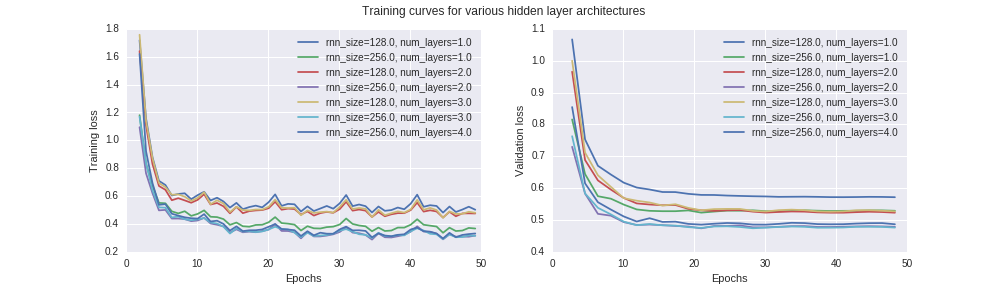
\includegraphics[width=\linewidth]{Figures/torch-rnn-network-params.png}
    \caption{torch-rnn-network-params}
    \label{fig:torch-rnn-network-params}
\end{figure}

Sensitivity to network structure: \texttt{num\_layers} and \texttt{rnn\_size}.
\begin{itemize}
    \item Larger \texttt{rnn\_size} leads to higher capacity and lower training loss
        \begin{itemize}
            \item Presents as overfitting on validation, where the lowest capacity
                model \texttt{rnn\_size} appears to be improving in generalization while
                others are flat/increasing
        \end{itemize}
    \item Training curves about the same wrt \texttt{num\_layers}, validation curves have interesting story
        \begin{itemize}
            \item Depth matters: small 64 and 128 hidden unit RNNs saw improvements up to 0.09
            \item Expressivity gained from depth furthers overfitting: 256
                hidden unit RNN has some of the best validation performance at
                depth 1 but is the worst generalizing model for depths 2
                and 3 even though training loss is low
        \end{itemize}
    \item \texttt{rnn\_size=128} undisputably best generalizing, optimized at
        \texttt{num\_layers=2}: will continue with these settings
\end{itemize}

\begin{figure}[htpb]
    \centering
    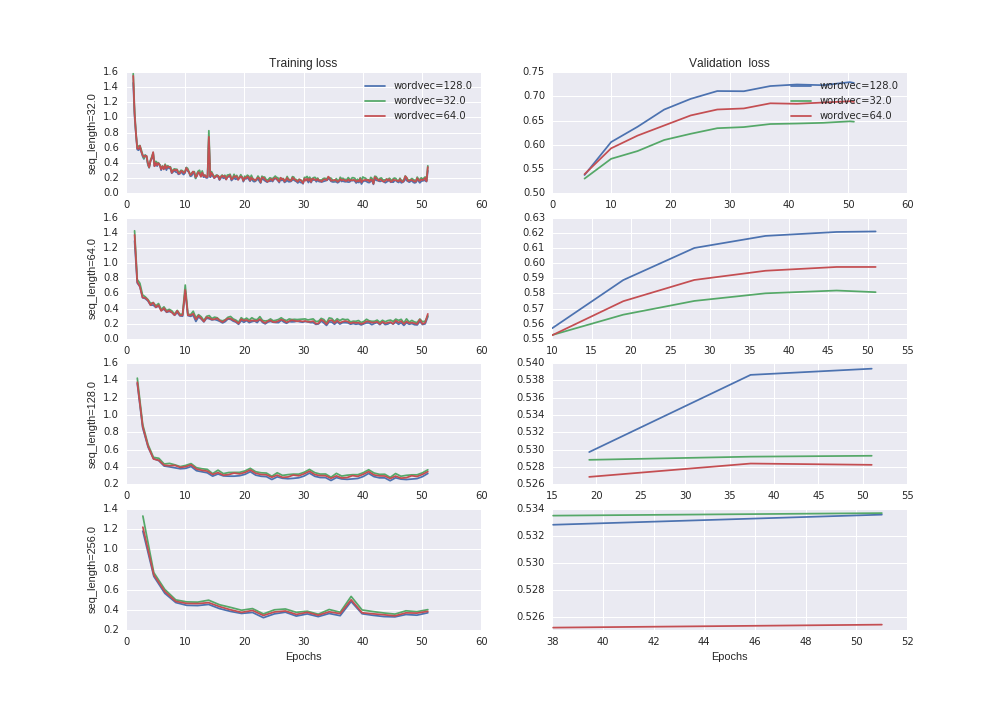
\includegraphics[width=\linewidth]{Figures/torch-rnn-input-params.png}
    \caption{torch-rnn-input-params}
    \label{fig:torch-rnn-input-params}
\end{figure}

Sensitivity to network inputs: \texttt{seq\_length} and \texttt{wordvec}
\begin{itemize}
    \item Training losses are about the same across all \texttt{wordvec}s
    \item Validation losses suggest that increasing \texttt{seq\_length} important for
        good performance \todo{investigate further}
    \item \texttt{wordvec=128} overfits for all cases, the other two depend on
        \texttt{seq\_length} and vary an order of magnitude smaller than the
        performance gains from increasing \texttt{seq\_length}
\end{itemize}

Data for all network configurations examined is available in \autoref{tab:torch-rnn-config-perfs}.

\begin{table}[htpb]
    \centering
    \caption{Performance of various LSTM configurations}
    \label{tab:torch-rnn-config-perfs}
    \begin{longtable}{rrrrrr}
\toprule
 num\_layers &  rnn\_size &  seq\_length &  wordvec &  train\_metric &  val\_metric \\
\midrule
\endhead
\midrule
\multicolumn{3}{r}{{Continued on next page}} \\
\midrule
\endfoot

\bottomrule
\endlastfoot
        2.0 &     128.0 &       128.0 &     64.0 &      0.296537 &    0.528261 \\
        2.0 &     128.0 &       128.0 &     32.0 &      0.316390 &    0.529308 \\
        2.0 &     128.0 &       128.0 &    128.0 &      0.273516 &    0.539359 \\
        3.0 &     128.0 &       128.0 &     32.0 &      0.265842 &    0.539827 \\
        1.0 &     256.0 &       128.0 &     32.0 &      0.285714 &    0.546995 \\
        3.0 &     128.0 &       128.0 &     64.0 &      0.247192 &    0.549826 \\
        1.0 &     128.0 &       128.0 &    128.0 &      0.360038 &    0.550509 \\
        1.0 &     128.0 &       128.0 &     64.0 &      0.384282 &    0.554990 \\
        1.0 &     256.0 &       128.0 &     64.0 &      0.238860 &    0.556672 \\
        3.0 &      64.0 &       128.0 &     64.0 &      0.420250 &    0.559336 \\
        3.0 &      64.0 &        64.0 &    128.0 &      0.345705 &    0.559549 \\
        3.0 &     128.0 &       128.0 &    128.0 &      0.238071 &    0.562603 \\
        2.0 &     256.0 &       128.0 &     32.0 &      0.143647 &    0.563866 \\
        2.0 &      64.0 &       128.0 &     64.0 &      0.443393 &    0.567754 \\
        1.0 &     128.0 &        64.0 &     32.0 &      0.359041 &    0.569011 \\
        3.0 &      64.0 &       128.0 &    128.0 &      0.408074 &    0.572306 \\
        1.0 &     128.0 &       128.0 &     32.0 &      0.417764 &    0.573797 \\
        2.0 &      64.0 &        64.0 &     32.0 &      0.413944 &    0.573993 \\
        3.0 &      64.0 &        64.0 &     64.0 &      0.355615 &    0.574236 \\
        1.0 &     256.0 &       128.0 &    128.0 &      0.204964 &    0.574585 \\
        1.0 &     128.0 &        64.0 &     64.0 &      0.328927 &    0.575464 \\
        2.0 &      64.0 &        64.0 &     64.0 &      0.390597 &    0.575592 \\
        2.0 &      64.0 &       128.0 &    128.0 &      0.424735 &    0.575868 \\
        2.0 &      64.0 &        32.0 &     32.0 &      0.399389 &    0.577974 \\
        2.0 &      64.0 &        64.0 &    128.0 &      0.372478 &    0.578856 \\
        2.0 &     128.0 &        64.0 &     32.0 &      0.240288 &    0.580802 \\
        3.0 &      64.0 &        64.0 &     32.0 &      0.375478 &    0.582072 \\
        1.0 &     128.0 &        64.0 &    128.0 &      0.304245 &    0.582897 \\
        3.0 &      64.0 &       128.0 &     32.0 &      0.430421 &    0.582991 \\
        3.0 &      64.0 &        32.0 &     32.0 &      0.348150 &    0.585800 \\
        2.0 &      64.0 &        32.0 &     64.0 &      0.387047 &    0.589173 \\
        3.0 &      64.0 &        32.0 &    128.0 &      0.339394 &    0.594401 \\
        1.0 &     128.0 &        32.0 &     32.0 &      0.348193 &    0.595001 \\
        2.0 &      64.0 &       128.0 &     32.0 &      0.470837 &    0.597005 \\
        3.0 &      64.0 &        32.0 &     64.0 &      0.344404 &    0.597406 \\
        2.0 &     128.0 &        64.0 &     64.0 &      0.224014 &    0.597418 \\
        1.0 &      64.0 &        32.0 &     64.0 &      0.462827 &    0.597437 \\
        1.0 &      64.0 &        32.0 &     32.0 &      0.500014 &    0.598521 \\
        2.0 &      64.0 &        32.0 &    128.0 &      0.376624 &    0.600570 \\
        1.0 &      64.0 &        32.0 &    128.0 &      0.453646 &    0.604043 \\
        2.0 &     256.0 &       128.0 &     64.0 &      0.122328 &    0.606237 \\
        1.0 &      64.0 &       128.0 &    128.0 &      0.489255 &    0.607122 \\
        1.0 &     128.0 &        32.0 &     64.0 &      0.319029 &    0.609441 \\
        1.0 &     128.0 &        32.0 &    128.0 &      0.294204 &    0.613838 \\
        1.0 &      64.0 &        64.0 &    128.0 &      0.436633 &    0.615036 \\
        1.0 &      64.0 &        64.0 &     64.0 &      0.461935 &    0.616265 \\
        2.0 &     128.0 &        64.0 &    128.0 &      0.206896 &    0.620845 \\
        2.0 &     256.0 &       128.0 &    128.0 &      0.106181 &    0.631364 \\
        3.0 &     128.0 &        64.0 &     32.0 &      0.185779 &    0.633145 \\
        1.0 &     256.0 &        64.0 &     32.0 &      0.200897 &    0.640652 \\
        1.0 &      64.0 &        64.0 &     32.0 &      0.487779 &    0.643943 \\
        2.0 &     128.0 &        32.0 &     32.0 &      0.209044 &    0.647553 \\
        1.0 &      64.0 &       128.0 &     64.0 &      0.515733 &    0.653191 \\
        1.0 &     256.0 &        64.0 &     64.0 &      0.171567 &    0.657626 \\
        3.0 &     256.0 &       128.0 &     64.0 &      0.087426 &    0.660995 \\
        3.0 &     128.0 &        64.0 &    128.0 &      0.169560 &    0.663409 \\
        3.0 &     128.0 &        64.0 &     64.0 &      0.172871 &    0.670402 \\
        1.0 &      64.0 &       128.0 &     32.0 &      0.561724 &    0.670482 \\
        1.0 &     256.0 &        64.0 &    128.0 &      0.149129 &    0.672432 \\
        3.0 &     256.0 &       128.0 &     32.0 &      0.093118 &    0.672697 \\
        2.0 &     128.0 &        32.0 &     64.0 &      0.193615 &    0.688310 \\
        3.0 &     256.0 &       128.0 &    128.0 &      0.076598 &    0.711632 \\
        2.0 &     256.0 &        64.0 &     32.0 &      0.081134 &    0.716840 \\
        2.0 &     128.0 &        32.0 &    128.0 &      0.173684 &    0.727354 \\
        2.0 &     256.0 &        64.0 &     64.0 &      0.073675 &    0.742250 \\
        1.0 &     256.0 &        32.0 &     32.0 &      0.161496 &    0.743529 \\
        3.0 &     128.0 &        32.0 &     32.0 &      0.146775 &    0.752404 \\
        1.0 &     256.0 &        32.0 &     64.0 &      0.138145 &    0.755407 \\
        1.0 &     256.0 &        32.0 &    128.0 &      0.125931 &    0.757801 \\
        3.0 &     128.0 &        32.0 &     64.0 &      0.134530 &    0.770094 \\
        2.0 &     256.0 &        64.0 &    128.0 &      0.063084 &    0.797383 \\
        3.0 &     128.0 &        32.0 &    128.0 &      0.129410 &    0.801131 \\
        3.0 &     256.0 &        64.0 &     64.0 &      0.048852 &    0.823713 \\
        3.0 &     256.0 &        64.0 &     32.0 &      0.052363 &    0.848516 \\
        2.0 &     256.0 &        32.0 &     32.0 &      0.058634 &    0.874037 \\
        3.0 &     256.0 &        64.0 &    128.0 &      0.044448 &    0.876398 \\
        2.0 &     256.0 &        32.0 &    128.0 &      0.049791 &    0.888397 \\
        2.0 &     256.0 &        32.0 &     64.0 &      0.050012 &    0.898488 \\
        3.0 &     256.0 &        32.0 &     32.0 &      0.037417 &    0.960396 \\
        3.0 &     256.0 &        32.0 &     64.0 &      0.034403 &    0.988554 \\
        3.0 &     256.0 &        32.0 &    128.0 &      0.036275 &    0.990457 \\
\end{longtable}

\end{table}

\section{Embeddings}

\subsection{Notes}

\begin{figure}[htpb]
    \centering
    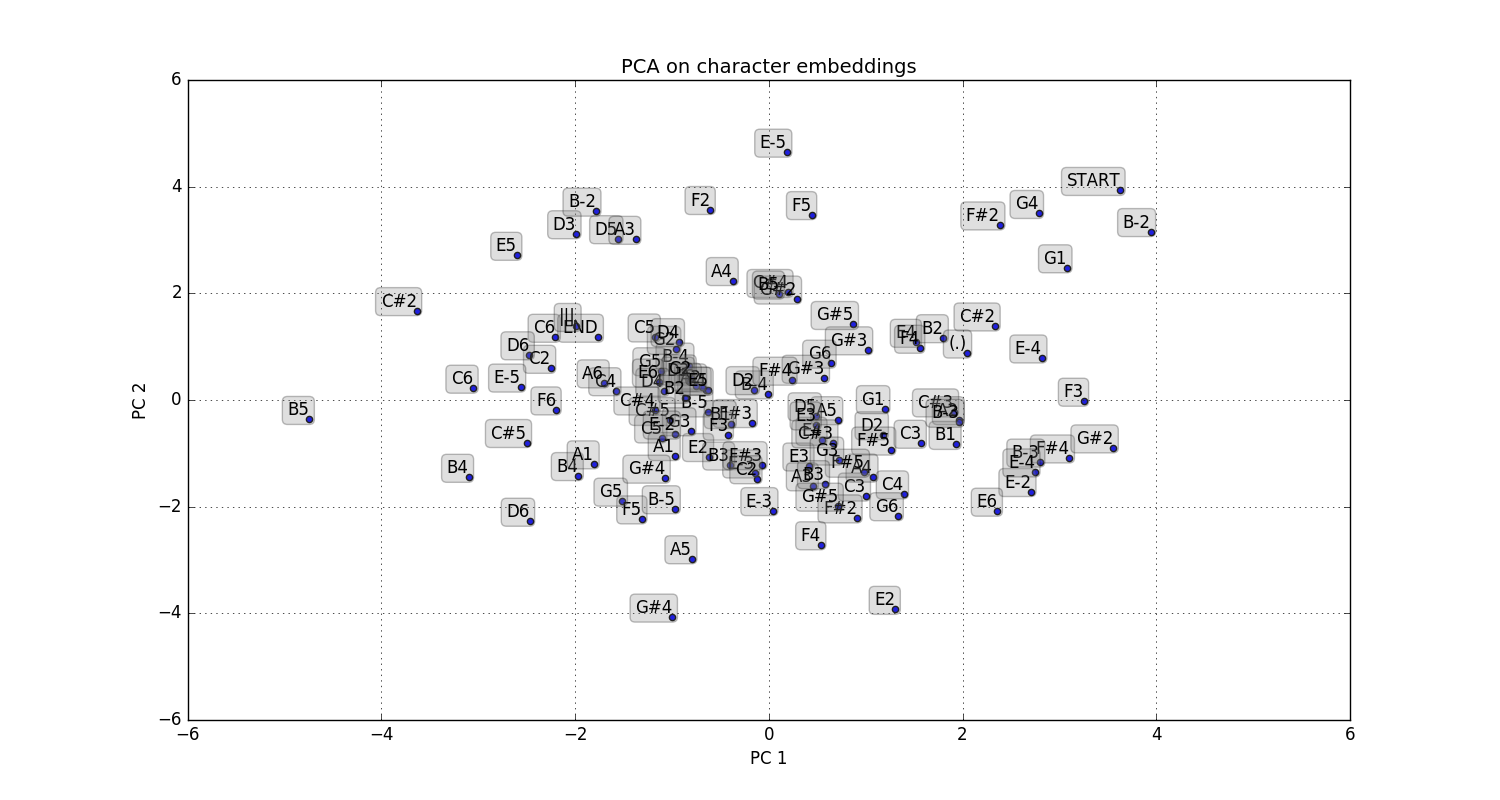
\includegraphics[width=0.8\linewidth]{Figures/PCA-notes.png}
    \caption{PCA embedding of note tokens}
    \label{fig:pca-notes}
\end{figure}

\begin{figure}[htpb]
    \centering
    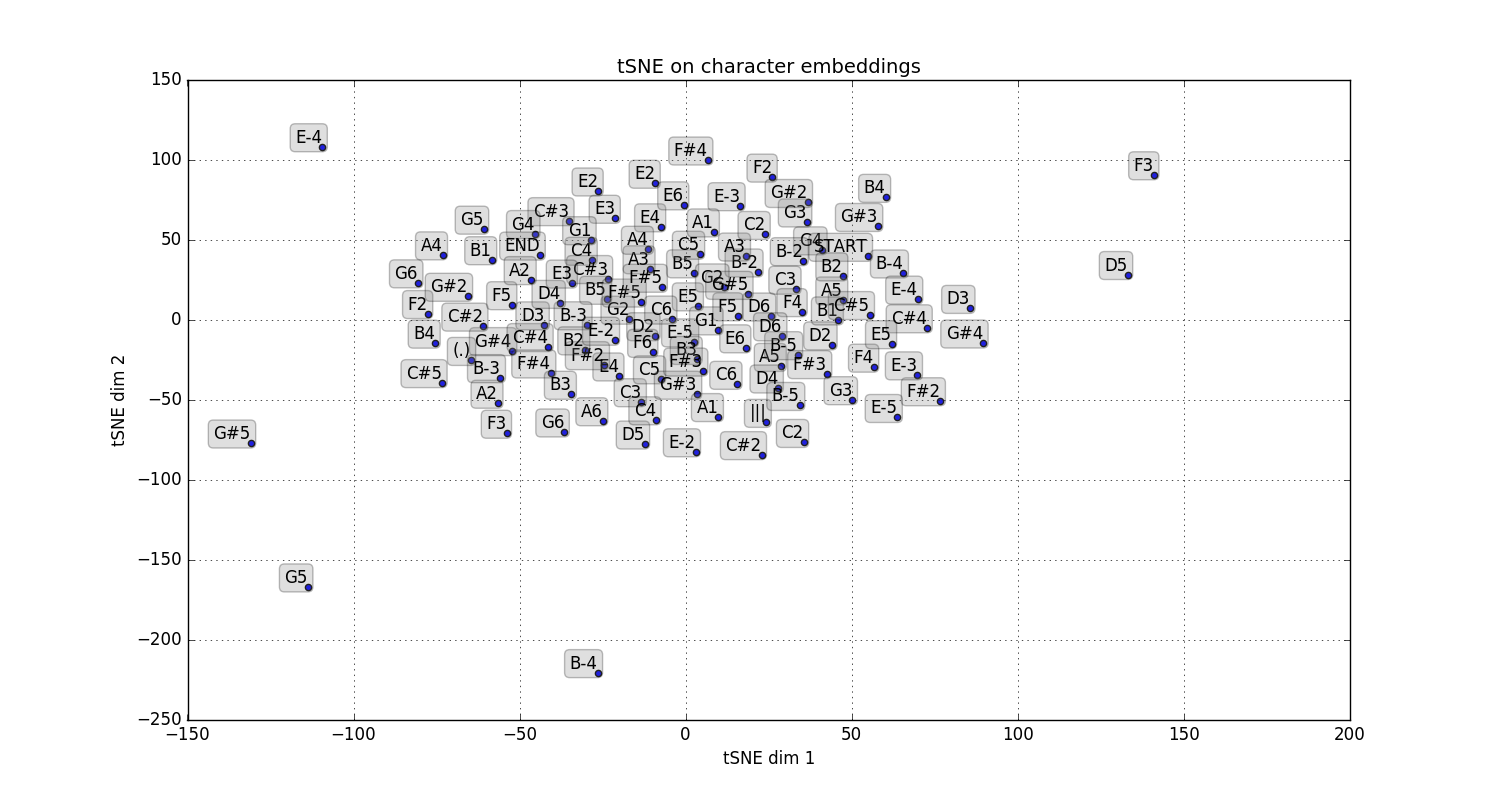
\includegraphics[width=0.8\linewidth]{Figures/tSNE-notes.png}
    \caption{tSNE embedding of note tokens}
    \label{fig:tsne-notes}
\end{figure}

\subsection{Chords}

\subsection{Phrases}

\subsection{Scores}

